\maketitle

\begin{abstract}\label{sec:abs}
SignMuon --- sign compression of the Muon update to one bit per parameter --- is the most straightforward adaptation of Muon to an extremely low communication budget. It outperforms SignSGD in practice, yet it can diverge on a linear function. The natural conjecture is that the order of operations is to blame, and that signing before rather than after the Linear Minimization Oracle (LMO) would fix it. It does not: MuonUSign diverges too, as does MuonSign, which signs both sides, so no naive placement of the sign around the LMO converges. Error feedback repairs one of them: EF21-MuonUSign attains the standard $\mathcal{O}(T^{-1/2})$ rate for smooth nonconvex optimization and decisively outperforms SignSGD, and compressing the downlink as well costs little beyond that. What the guarantee costs is the placement. Across centralized, federated and language-modelling experiments the best placement is consistently sign-\emph{after}-the-LMO, precisely the one our counterexamples break and error feedback fails to repair. The provably convergent sign-before variants trail it by about two accuracy points in federation. We report this tension rather than resolve it: the counterexamples constrain worst-case instances, not CIFAR-10.
\end{abstract}


% \textbf{Keywords:} federated learning, stochastic optimization, gradient compression, 1-bit quantization, matrix orthogonalization, LMO, SignSGD, Muon.


\section{Introduction}\label{sec:intro}
Training a deep network across clients costs bandwidth as well as computation: every round, each client must ship a full update, and under a limited link those updates dominate the wall-clock cost. Compression is the standard remedy \cite{bernstein2018signsgd, bernstein2019signsgdmajority, beznosikov2020biased}, and SignSGD is its extreme point: one bit per coordinate, at little cost in final accuracy. But SignSGD flattens each weight matrix into a vector, discarding the two-dimensional structure that matrix-aware optimizers exploit. Muon exploits precisely that structure: it orthonormalizes the momentum matrix before stepping, which stabilizes training and, in several settings, beats tuned adaptive methods \cite{jordan2024muon, bernstein2024old, shah2025practical}. What it sends, however, is a \emph{dense} matrix at full precision --- the one thing a bandwidth-limited system cannot afford. Matrix geometry and a one-bit budget pull in opposite directions.

% In this work, we propose SignMuon,
% % \footnote{Code is available at: \url{https://github.com/intsystems/2026-Project-203/tree/main}},
% an optimization algorithm that applies sign compression to the Linear Minimization Oracle (LMO) update of Muon. SignSGD transmits the sign of the coordinates of the stochastic gradient direction. Our algorithm first computes an update direction using LMO, and then transmits only the sign of this direction. This approach allows for the matrix structure of the parameters to be accounted for and preserves the advantages of Muon, while reducing the amount of transmitted information to one bit per coordinate. Consequently, SignMuon combines the fast convergence of structured optimizers with the communication efficiency of sign-based approaches.
We study the natural ways to combine sign compression with the Muon LMO at one bit per parameter: \textbf{SignMuon}, which signs \emph{after} the LMO, $\operatorname{sign}(\operatorname{LMO}(\cdot))$; \textbf{MuonUSign}, which signs \emph{before}, $\operatorname{LMO}(\operatorname{sign}(\cdot))$; and \textbf{MuonSign}, which signs on \emph{both} sides and so compresses uplink and downlink alike. All three keep Muon's matrix-aware geometry, but only sign-after reaches Muon's accuracy: at $N=11$ clients the three span five accuracy points, in the order after, before, both sides, the last of them falling below SignSGD.

None of them, however, has a global convergence guarantee. We prove that all three can diverge: SignMuon on a $4\times4$ instance (Theorem~\ref{th:1}), MuonUSign and MuonSign on a single common $5\times5$ one (Theorems~\ref{th:2}--\ref{th:3}). In each case the 1-bit step becomes an ascent direction on a linear objective. To restore convergence at the same communication volume we introduce \textbf{EF21-MuonUSign}, adapted from EF21-Muon~\citep{gruntkowska2025error}: the scaled sign compresses only the residual between the momentum and a gradient estimator, and the descent step takes the full Muon LMO of the reconstructed estimator. \textbf{EF21-MuonSign} adds a second error-feedback loop on the downlink, compressing both channels to one bit. Both descend on the counterexamples above.

% The effectiveness of the proposed optimizer is evaluated on synthetic and practical tasks: centralized image classification on CIFAR-10 with a ResNet-18 backbone, federated image classification on CIFAR-10 with a CNN across several client counts, and on a synthetic smooth convex least-squares problem.
We evaluate the methods on centralized CIFAR-10 with a ResNet-18, federated CIFAR-10 with a CNN at $N=11$ clients, the nanoGPT speedrun, and a synthetic smooth convex least-squares problem. Our contributions are: (i)~SignMuon, MuonUSign and MuonSign, matrix-aware 1-bit optimizers placing the sign after, before and on both sides of the LMO; (ii)~counterexamples proving all three may diverge (Theorems~\ref{th:1}--\ref{th:3}), at essentially minimal matrix sizes; (iii)~a universal divergence theorem (Theorem~\ref{th:ef_div}): error feedback on the LMO \emph{output} repairs SignMuon for no $(L,\eta,\mu)$; (iv)~EF21-MuonUSign, restoring the guarantee at a one-bit uplink, and (v)~EF21-MuonSign, adding a downlink loop to keep both channels at one bit; and (vi)~a tuned five-seed federated comparison of all six at one budget, separating the three placements single-seed evidence had shown as coincident and locating the guarantee's cost at the placement, not the downlink. Proofs, algorithms, and the numbered results cited but not stated below are in the supplementary material.

% Experimental results show that applying sign compression to Muon directions reduces communication overhead (by $32\times$) while maintaining optimization rates. In the centralized setting, SignMuon consistently outperforms the baseline SignSGD method in both convergence speed and final accuracy. At the same time, the accuracy of the proposed 1-bit method is only $1-1.5\%$ lower than that of the Muon optimizer, while significantly outperforming basic signed algorithms. In federated setting, integrating SignMuon with client momentum and Majority Vote aggregation method provides stable convergence and robustness to anomalous client updates even under severe communication constraints. Furthermore, we present an analytical example that formalizes the limitations of applying sign compression to LMO-based updates in the deterministic setting and for smooth convex optimization problems. The results of our experiments demonstrate that the proposed algorithm successfully combines LMO-based methods with sign compression without any significant loss in training accuracy.

\section{Related Work}\label{sec:relWork}
\paragraph{SignSGD.} Vanilla SignSGD, introduced by \citet{bernstein2018signsgd} and later applied to federated learning by \citet{bernstein2019signsgdmajority}, required increasing batch sizes to guarantee convergence. This issue, together with SignSGD's inherent bias, was addressed through the adoption of the Error Feedback technique \citep{karimireddy2019efsign}. An alternative approach is to randomize the sign operator itself \citep{chen2020median,safaryan2021ssdm,jin2024stosign}.

\paragraph{Compression for Muon.} \citet{gruntkowska2025error} developed a theoretical framework for federated learning with error feedback in which Muon/Gluon \citep{riabinin2025gluon} updates are compressed bidirectionally (client-to-server and server-to-client). \citet{qian2026communicationefficientgluon} employed variance reduction to lower the compression error for Gluon under unbiased and contractive compressors. Concurrently with our work, \citet{mishra2026signmuon} proposed vanilla SignMuon and stated an $\mathcal{O}(1/\sqrt{T})$ guarantee for it; in Appendix~\ref{app:mishra} we show that their finalized rate covers only the gradient-sign instantiation, leaving the bound for the actual polar-sign method uninformative on exactly the instances of Theorem~\ref{th:1}. Two further methods share our names but not our object: \citet{bolatov2026lionmuon} \emph{alternate} spectral and sign steps instead of composing them, and \citet{kravatskiy2025kyfannorms} mix the two geometries \emph{inside} the oracle, so S-Muon remains an LMO for an explicit norm and keeps the attendant theory. Our three placements put the sign \emph{around} the oracle, where it is a compressor and not a geometry, so the counterexamples below do not bear on either (Appendix~\ref{app:smuon}).

\section{Problem Statement}\label{sec:proState}

We consider the stochastic optimization problem
\begin{equation}
\min_{\mathbf{X} \in \mathcal{X}} \{f(\mathbf{X}) := \mathbb{E}_{\xi \sim \mathcal{D}} [f_{\xi}(\mathbf{X})]\},
\end{equation}
where $\mathcal{X}$ is the parameter space (e.g., $\mathbb{R}^d$ or $\mathbb{R}^{m \times n}$) and the $f_{\xi} : \mathcal{X} \to \mathbb{R}$ are continuously differentiable and possibly non-convex: $f_{\xi}(\mathbf{X})$ is the loss of a model $\mathbf{X}$ at a data point $\xi \sim \mathcal{D}$. In the federated setting the data are split across clients, and the training problem becomes

\begin{multline}
\min_{\mathbf{X} \in \mathcal{X}} \left\{ f(\mathbf{X}) := \frac{1}{N}\sum_{j=1}^N f_j(\mathbf{X})\right\}, \\
f_j(\mathbf{X})=\mathbb{E}_{\xi_j\sim\mathcal{D}_j}[f_j(\mathbf{X};\xi_j)]
\label{fed_eq}
\end{multline}
where $N \ge 1$ is the number of clients and $f_j$ is the loss on the data $\mathcal{D}_j$ held by client $j \in [N] := \{1, \dots, N\}$.

Two assumptions run through the paper. The model is a tuple of matrix layers $\mathbf{X} = [\mathbf{X}_1,\dots,\mathbf{X}_p]$, $\mathbf{X}_i \in \mathbb{R}^{m_i\times n_i}$, with $\nabla_i$ the gradient block of layer $i$. Each layer carries the spectral norm $\|\cdot\|_{2\to2}$, whose dual is the nuclear norm $\|\cdot\|_{*}$, and we write $\|\nabla f(\mathbf{X})\|_*^2 := \sum_i\|\nabla_i f(\mathbf{X})\|_*^2$; a single matrix parameter is the case $p=1$.

\begin{assumption}[\textbf{Lower boundedness}]\label{as:1}
$f(\mathbf{X}) \ge f^*$ for all $\mathbf{X}$; where explicitly invoked, each local $f_j \ge f_j^*$ as well.
\end{assumption}

\begin{assumption}[\textbf{Layer-wise smoothness}]\label{as:2}
For every layer $i$ and all $\mathbf{X},\mathbf{Y}$,
\begin{equation}
\|\nabla_i g(\mathbf{X}) - \nabla_i g(\mathbf{Y})\|_{*} \le L_i^{g}\,\|\mathbf{X}_i - \mathbf{Y}_i\|_{2\to 2}
\end{equation}
for $g = f$ (constant $L_i$) and $g = f_j$ (constant $L_{i,j}$). A weaker layer-wise $(L^0,L^1)$ form, stated in Appendix~\ref{app:prelim}, is used only in Corollary~\ref{cor:l0l1}.
\end{assumption}

A Linear Minimization Oracle (LMO) minimizes a linear form over the unit ball of a norm, returning the steepest-descent direction in that norm (Appendix~\ref{app:prelim}). Muon takes that norm to be spectral on each matrix layer, which turns the oracle into an orthogonalization: writing $\mathbf{M}=\mathbf{U}\boldsymbol{\Sigma}\mathbf{V}^\top$ for the rank-$r$ singular value decomposition of $\mathbf{M}\in\mathbb{R}^{m\times n}$, the LMO direction is
\begin{equation}
A(\mathbf{M})=-\mathbf{U}\mathbf{V}^\top \in \mathbb{R}^{m\times n},
\qquad \operatorname{polar}(\mathbf{M}):=-A(\mathbf{M}).
\end{equation}
In practice the oracle is applied to a momentum estimate rather than to $\mathbf{G}_t$ itself; \eqref{eq:signa_general} below gives the full iteration.

Muon requires transmitting the full update matrix $\mathbf{D}_t$, which is expensive in federated settings. Our objective is to combine its matrix-aware geometry with extreme (1-bit) communication compression. SignMuon, MuonUSign, and MuonSign achieve it empirically, but lack global convergence guarantees (Theorems~\ref{th:1}--\ref{th:3}). The Error-Feedback variants restore convergence: in Appendix~\ref{app:hyp} we show that EF21-MuonUSign and EF21-MuonSign are \emph{exact instances} of the EF21-Muon framework of \citet{gruntkowska2025error}, and so inherit the standard $\mathcal{O}(T^{-1/2})$ rate for smooth non-convex optimization (Theorem~\ref{thm:conv}):
\begin{equation}
\min_{0 \le t \le T}\mathbb{E}\bigl[\|\nabla f(\mathbf{X}_t)\|_*^2\bigr]
= \mathcal{O}(T^{-1/2}),
\end{equation}
as well as an $\mathcal{O}(T^{-1/4})$ rate for $\min_t \sum_i \mathbb{E}\|\nabla_i f(\mathbf{X}_t)\|_*$ under $(L^0,L^1)$-smoothness with a plain constant learning rate (Corollary~\ref{cor:l0l1}). Both displays assume one step-size constant common to all layers; Corollaries~\ref{cor:smooth}--\ref{cor:l0l1} give the general weighted form. Finally, EF21-MuonSign adds a second error-feedback loop on the downlink, making communication 1-bit in \emph{both} directions. The $\mathcal{O}(T^{-1/2})$ rate survives, but not without cost: a sign-based downlink is contractive only in the Euclidean norm, whereas Muon's spectral geometry asks for contractivity in the layer norm, so the admissible step size shrinks by a further $\sqrt{r}$ in the layer rank. The gap is not an artefact of the analysis: the scaled sign is spectrally contractive for \emph{no} parameter at all, so only a different compressor helps (Remark~\ref{rem:normmismatch}). We measure what it costs on a transformer (Section~\ref{sec:exp_nanogpt}).


\section{Theory}\label{sec:theory}
Consider the \textbf{SignA} family, where A is any optimizer built on LMO directions. A SignA method initializes $\mathbf{M}_0 = \mathbf{0}$ and at each iteration $t \ge 1$ performs:
\begin{equation}
\label{eq:signa_general}
\resizebox{0.98\columnwidth}{!}{\(\displaystyle
\begin{aligned}
\mathbf{M}_t &= \mu \mathbf{M}_{t-1} + \mathbf{G}_t & \text{(Momentum accumulation)}\\
\tilde{\mathbf{M}}_t &=
\begin{cases}
    \mathbf{G}_t + \mu \mathbf{M}_t & \text{(Nesterov momentum)}, \\
    \mathbf{M}_t & \text{(otherwise)}
\end{cases} & \text{(Effective direction)}, \\
\mathbf{D}_t &= -A(\tilde{\mathbf{M}}_t), & \text{(LMO direction)} \\
\mathbf{s}_t &= \operatorname{sign}(\mathbf{D}_t) \in \{\pm 1\}^{m \times n},  & \text{(Sign compression)}\\
\mathbf{X}_{t+1} &= \mathbf{X}_t - \eta_t \mathbf{s}_t & \text{(Parameter update)},
\end{aligned}\)}
\end{equation}
where $\mathbf{X}_t \in \mathbb{R}^{m \times n}$ is the parameter matrix, $\mathbf{G}_t$ its stochastic gradient, $\mu \in [0, 1)$ the momentum coefficient and $\eta_t$ the learning rate; $A(\cdot)$ is the LMO, and $\operatorname{sign}(\cdot)$ acts element-wise on the structured direction $\mathbf{D}_t$, with $\operatorname{sign}(0)$ resolved to an independent random $\pm1$ so that the transmitted alphabet stays binary.

Our three methods are the three placements of the sign around this oracle. They share the update $\mathbf{X}_{t+1}=\mathbf{X}_t-\eta_t\,\mathbf{s}_t$ and differ only in where the sign acts on $\tilde{\mathbf{M}}_t$:
\begin{equation}
\label{eq:three_placements}
\mathbf{s}_t=
\begin{cases}
\operatorname{sign}\!\bigl(\operatorname{polar}(\tilde{\mathbf{M}}_t)\bigr) & \text{(SignMuon: after)},\\[2pt]
\operatorname{polar}\!\bigl(\operatorname{sign}(\tilde{\mathbf{M}}_t)\bigr) & \text{(MuonUSign: before)},\\[2pt]
\operatorname{sign}\!\bigl(\operatorname{polar}(\operatorname{sign}(\tilde{\mathbf{M}}_t))\bigr) & \text{(MuonSign: both)}.
\end{cases}
\end{equation}
SignMuon (Algorithm~\ref{central_alg}) thus combines Muon's orthogonalized direction with the sign compression of SignSGD, MuonUSign (Algorithm~\ref{alg:muon_usign}) signs before the oracle instead, and MuonSign (Algorithm~\ref{alg:muon_sign}) signs both sides. All three transmit one bit per parameter on the uplink. On the downlink SignMuon and MuonSign distribute a $\pm1$-valued object and so cost one bit in each direction, while MuonUSign's server-side $\operatorname{polar}(\cdot)$ is dense and costs full precision.

\subsection{Centralized Learning}
% In the centralized setting, SignMuon is applied to the matrix-valued parameters of a neural network. The practical implementation takes into account the tensor structure of model parameters. The optimization process is divided into two separate streams: matrix parameters (weights of convolutional and fully connected layers, $n_{dim} \ge 2$) are updated using the SignMuon LMO-based procedure, whereas vector parameters (bias, Batch Normalization layer, $n_{dim} = 1$) as well as the final classification layer are optimized using the standard AdamW optimizer. This design was originally introduced in the empirical description of Muon by \citet{jordan2024muon}. The first theoretical convergence result was derived by Li and Hong, who analyzed the smooth non-convex setting \cite{li2025note} and subsequently formalized within the Gluon framework \cite{riabinin2025gluon}.
In the centralized setting, SignMuon is applied to the matrix-valued parameters (weights of convolutional and fully connected layers, $n_{dim}\ge 2$), while vector parameters (biases, BatchNorm, $n_{dim} = 1$) and the final classification layer are optimized with AdamW, the design introduced by \citet{jordan2024muon} and formalized in \cite{li2025note, riabinin2025gluon}.

We approximate $\operatorname{polar}(\cdot)$ by a 5th-order Newton--Schulz iteration rather than a full SVD at every step (Algorithm~\ref{alg:muon_lmo}). One further implementation choice is not without consequence, and we state it here because every experiment depends on it.

\paragraph{Per-layer step sizes: the unit-gain heuristic.} The methods of this paper produce step matrices from two families with \emph{exactly} known Frobenius norms: $\|\mathbf{U}\mathbf{V}^\top\|_F=\sqrt{r}$ for the \textsc{lmo}-terminated methods ($r=\min(m,n)$), and $\|\mathbf{s}\|_F=\sqrt{mn}$ for the \textsc{sign}-terminated ones. These scale differently with layer shape, so no single global $\eta$ is right for both families, or across layers within one. We fix the shape dependence a priori and tune only a shape-free base rate $\eta_0$, setting $\eta_\ell=\eta_0\lambda_\ell$ with
\begin{equation}
\label{eq:unit_gain_main}
\lambda_\ell=\frac{\sqrt{m}}{\|\mathbf{s}_\ell\|_F}
\quad\Longrightarrow\quad
\begin{cases}
\lambda_\ell^{\textsc{lmo}}=\sqrt{\max(1,m/n)},\\[2pt]
\lambda_\ell^{\textsc{sign}}=1/\sqrt{\text{fan-in}}.
\end{cases}
\end{equation}
The criterion is that every layer's update have the same root-mean-square input--output gain, the average-case form of the spectral scaling condition \citep{yang2023spectral,large2024modular}; $\eta_0$ is then literally the per-step RMS gain. We treat \eqref{eq:unit_gain_main} as a heuristic and use it uniformly, for one reason above all: its \textsc{lmo} branch \emph{reproduces} the aspect-ratio factor $\sqrt{\max(1,m/n)}$ that the reference Muon implementation already ships as a practical fix \citep{jordan2024muon}, so a criterion already accepted in practice for one family supplies the missing counterpart, $1/\sqrt{\text{fan-in}}$, for the other. Appendix~\ref{app:lrscale} gives the derivation, the measurement that selects the exponent $\tfrac12$ over $\mu$P's $1$, the caveats, and the sensitivity of our conclusions to the choice.

% Declared ahead of its first reference below: a two-column float can only
% move forward on the page, and from the next subsection it would land a
% page after the text that discusses it.
\begin{figure*}[!t]
    \centering
    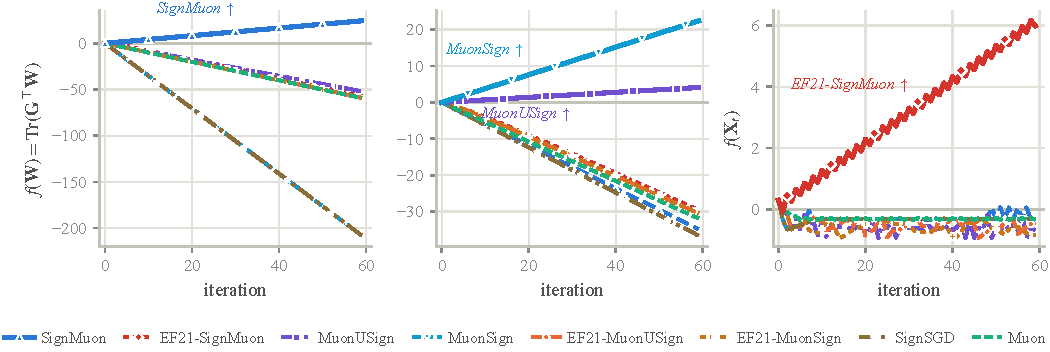
\includegraphics[width=\textwidth]{images/counterexamples/counterexamples_main.pdf}
    \caption{All eight methods on the three counterexample instances; in each panel the ascending method is drawn heavy and named. \emph{Left:} SignMuon on the $4\times4$ instance of Theorem~\ref{th:1}. \emph{Centre:} MuonUSign and MuonSign on the shared $5\times5$ instance of Theorems~\ref{th:2}--\ref{th:3}; both panels plot the linear objective~\eqref{eq:lin_obj}. \emph{Right:} EF21-SignMuon on the $2\times2$ instance of Theorem~\ref{th:ef_div}, in normalized units with $\eta=1$. Trajectories are momentum-free: for the three placements Proposition~\ref{prop:reduction} shows this is without loss, and for EF21-SignMuon Lemma~\ref{lem:efsm_realize} supplies a separate instance per $(\mu,\text{variant})$ generating the same target sequence; the remaining baselines are shown at $\mu=0$ only.}
    \label{fig:divergence_plot}
\end{figure*}

\subsection{Theoretical limitations}
A natural hope is that the Muon LMO direction --- the steepest-descent direction in the spectral norm --- survives sign compression, whether the sign is applied before or after the oracle. It does not: in each of the three placements the compressed step can become an \emph{ascent} direction on a smooth objective.

We read $\operatorname{polar}(\cdot)$ off the rank-truncated SVD. At a rank-deficient argument the spectral-ball LMO is not unique, and this selection, the one our implementation makes, is part of what the counterexamples assert.

We refute the descent property on \emph{linear} objectives (the simplest smooth functions, on which any sound method must make unbounded progress):
\begin{equation}
\label{eq:lin_obj}
f(\mathbf{W})=\langle \mathbf{G},\mathbf{W}\rangle=\operatorname{Tr}(\mathbf{G}^\top\mathbf{W}),\qquad \nabla f(\mathbf{W})\equiv \mathbf{G}.
\end{equation}
Gradient descent and full-precision Muon drive $f\to-\infty$ here, so a rule that instead drives $f\to+\infty$ is unambiguously ascending (Remark~\ref{rem:efsm_bdd} restores Assumption~\ref{as:1} without moving any trajectory below).

On \eqref{eq:lin_obj} the step is the constant matrix $\mathbf{s}(\mathbf{G})$ whatever the momentum, so momentum affects neither convergence nor divergence (Proposition~\ref{prop:reduction}, Appendix~\ref{app:proof_reduction}) and
\begin{equation}
\label{eq:lin_increment}
f(\mathbf{X}_{t+1})-f(\mathbf{X}_t)=-\eta_t\,\bigl\langle \mathbf{G},\ \mathbf{s}(\mathbf{G})\bigr\rangle
\end{equation}
for every $\mu\in[0,1)$ and either momentum rule. One gradient with $\langle\mathbf{G},\mathbf{s}(\mathbf{G})\rangle<0$ thus makes $f$ increase at \emph{every} step, at \emph{any} step size, with $f(\mathbf{X}_t)\to+\infty$ whenever $\sum_t\eta_t=\infty$.

Such a gradient exists for each placement: a $4\times4$ matrix defeats SignMuon, and a single $5\times5$ matrix defeats MuonUSign and MuonSign together. Informally, then:

\begin{quote}
For each of the three placements there is a linear objective on which the method ascends at every iteration, for every step size, every $\mu\in[0,1)$ and either momentum variant.
\end{quote}

These are Theorems~\ref{th:1}--\ref{th:3}, stated with their instances and proved in Appendices~\ref{app:proof_th1}--\ref{app:proof_th3}, which also show the sizes to be minimal. The left and centre panels of Figure~\ref{fig:divergence_plot} show the ascents. No placement of the sign around the Muon LMO, then, yields a convergent method.

\subsection{Centralized Error Feedback: EF21-SignMuon}

Theorems~\ref{th:1}--\ref{th:3} rule out every static placement of the sign around the LMO. The classical remedy for a biased one-bit compressor is \emph{error feedback}: store the compression error and reinject it at the next step. This repairs SignSGD~\cite{karimireddy2019efsign} and was later sharpened into EF21~\cite{richtarik2021ef21}. Its most direct use for SignMuon keeps the geometry (the sign \emph{after} the LMO) and error-feedbacks the oracle's output. The resulting method, \textbf{EF21-SignMuon} (Algorithm~\ref{ef21_signmuon}), tracks an estimate $\mathbf{d}_t^{\mathrm{est}}$ of the LMO direction $\mathbf{D}_t=\operatorname{polar}(\tilde{\mathbf{M}}_t)$, refreshed by a scaled sign of the residual,
\begin{equation}\label{eq:efsm_est}
\begin{aligned}
\mathbf{d}_t^{\mathrm{est}}&=\mathbf{d}_{t-1}^{\mathrm{est}}+\alpha_t\operatorname{sign}\!\bigl(\mathbf{D}_t-\mathbf{d}_{t-1}^{\mathrm{est}}\bigr),\\
\alpha_t&=\operatorname{mean}\bigl|\mathbf{D}_t-\mathbf{d}_{t-1}^{\mathrm{est}}\bigr|,
\end{aligned}
\end{equation}
and steps $\mathbf{X}_t=\mathbf{X}_{t-1}-\eta_t\,\mathbf{d}_t^{\mathrm{est}}$.

Error feedback on the compressed \emph{output}, however, does not restore the descent property, and fails for \emph{every} step size and momentum setting.
% The three divergence theorems are now stated in the appendix, next to their
% proofs, but the paper's numbering is fixed by everything that cites it (the
% code, its READMEs, the reproduction guide): Theorems 1-3 are the three sign
% placements, 4 is this one, 5 is the convergence result. The counter is set by
% hand here and reset in the appendix to keep those numbers.
\setcounter{theorem}{3}
\begin{theorem}[Divergence of EF21-SignMuon]\label{th:ef_div}
For every $L>0$, step size $\eta>0$, momentum coefficient $\mu\in[0,1)$, and either momentum variant, there is an $L$-smooth (Assumption~\ref{as:2}), bounded-below (Assumption~\ref{as:1}) function $f:\mathbb{R}^{2\times2}\!\to\mathbb{R}$ on which EF21-SignMuon started at $\mathbf{X}_0=\mathbf{0}$ diverges: for an explicit constant $c=c(f)>0$,
\begin{equation}\label{eq:exact_rate}
f(\mathbf{X}_{t+2})-f(\mathbf{X}_t)=c\,L\eta^2>0\qquad(t\ge3),
\end{equation}
so $f(\mathbf{X}_t)\to+\infty$. In particular, no step-size rule $\eta=\eta(L,\mu)$ using only the smoothness and momentum constants can make the method convergent.
\end{theorem}
The obstruction (proof in Appendix~\ref{app:proof_th4}) is specific to signing the LMO output: a \emph{single} magnitude $\alpha_t$ rescales all entries' signs at once, so a large, sign-flipping off-diagonal forces $\alpha_t=\Theta(1)$ and overwhelms the small diagonal target, whose estimate then locks onto the \emph{wrong} sign and drives one coordinate of $\mathbf{X}_t$ to infinity. Momentum does not help: Figure~\ref{fig:ef21_momentum} (Appendix~\ref{app:proof_th4}) records the same rate for every $\mu$ and both variants. The remedy is to error-feedback the gradient \emph{before} the LMO, the subject of the next subsection.

\subsection{Centralized Error Feedback: EF21-MuonUSign and EF21-MuonSign}
The defect is not the shared magnitude $\alpha_t$ as such, since the methods below couple all coordinates through the same scalar; it is \emph{what the estimator is asked to track}. Error feedback needs a target that settles, whereas the LMO output $\operatorname{polar}(\tilde{\mathbf{M}}_t)$ is non-Lipschitz in the momentum and can jump by $\Theta(1)$ between rounds however small $\eta$ is. Compressing the \emph{gradient} instead leaves the estimator tracking a target that moves with the step size, which restores convergence at the same one-bit uplink cost; we adapt the EF21-Muon mechanism~\cite{gruntkowska2025error} to sign compression.

The \textbf{USign} compressor is the directional pair $(\mathcal{C}_{\uparrow},\mathcal{C}_{\downarrow})$ with $\mathcal{C}_{\uparrow}(\mathbf{Y}) = \operatorname{mean}|\mathbf{Y}|\,\operatorname{sign}(\mathbf{Y})$ the scaled sign on the uplink and $\mathcal{C}_{\downarrow} = I$ the identity on the downlink: one bit per parameter from client to server, a full-precision model back. \textbf{EF21-MuonUSign} pairs it with EF21 and the Muon LMO.

EF21-MuonUSign maintains a gradient estimator $\mathbf{g}_t^{\mathrm{est}}$ updated via a contractive sign compressor on the residual $\Delta_t = \mathbf{M}_t - \mathbf{g}_t^{\mathrm{est}}$:
\begin{equation}
\alpha_t = \operatorname{mean}(|\Delta_t|),\quad
\mathbf{g}_{t+1}^{\mathrm{est}} = \mathbf{g}_t^{\mathrm{est}} + \alpha_t\,\operatorname{sign}(\Delta_t),
\label{eq:ef21_central}
\end{equation}
and takes the descent step
\begin{multline}
\mathbf{X}_{t+1} = \mathbf{X}_t - \eta_t\,\,\mathbf{D}_t,
\\ \mathbf{D}_t = -A(\mathbf{g}_{t+1}^{\mathrm{est}}) \approx \mathbf{U}_{t+1}\mathbf{V}^\top_{t+1}.
\label{eq:ef_step}
\end{multline}
Here $\mathbf{U}_{t+1}\mathbf{V}_{t+1}^\top$ is the polar factor of the estimator, not of $\nabla f$, so no step-wise descent property is claimed; what it provides is an estimator tracking a target that moves at the step size, the hypothesis the transferred guarantee needs (Corollary~\ref{cor:smooth}). The sign in~\eqref{eq:ef21_central} acts only on the internal compression residual, so the uplink stays at one bit per parameter (Algorithm~\ref{central_alg_ef}, Appendix~\ref{app:alg}). Figure~\ref{fig:divergence_plot} confirms that EF21-MuonUSign descends on the counterexample on which SignMuon ascends.

\textbf{EF21-MuonSign} makes both channels one-bit by applying the same scaled-sign operator to the downlink. The mechanism is a second error-feedback loop, on the \emph{model} rather than the gradient, and it splits the method into two iterates:
\begin{equation}\label{eq:two_models}
\begin{aligned}
  \mathbf{X}_{t+1}&=\mathbf{X}_t-\eta_t\mathbf{D}_t &&\text{(server model)},\\
  \mathbf{W}_{t+1}&=\mathbf{W}_t+\alpha_t^{\downarrow}\operatorname{sign}(\mathbf{X}_{t+1}-\mathbf{W}_t) &&\text{(broadcast model)},
\end{aligned}
\end{equation}
with $\mathbf{D}_t=-A(\mathbf{g}_{t+1}^{\mathrm{est}})$ as before. The server model $\mathbf{X}$ takes the exact LMO step and never leaves the server; what crosses the downlink is the one-bit refresh of the broadcast model $\mathbf{W}$, and $\mathbf{W}$ is the only model the rest of the method ever sees. Gradients, momentum and the uplink residual are all computed there. Training takes place at $\mathbf{W}$; the transferred guarantee (Corollary~\ref{cor:smooth}) bounds the gradient at $\mathbf{X}$. Under an exact downlink the two coincide and the method reduces to EF21-MuonUSign; how far they drift apart under the one-bit downlink is measured in Section~\ref{sec:exp_nanogpt}. The full procedure is Algorithm~\ref{central_alg_ud}; centrally the ``channels'' are internal to the update rule, which simply maintains both matrices.

Both error-feedback methods incur a memory cost for the guarantee: one buffer per compressed channel (the gradient estimate $\mathbf{g}^{\mathrm{est}}$; for EF21-MuonSign also the broadcast model $\mathbf{W}$). The overhead is small on the server but may be unwanted on memory-limited workers.


\subsection{Federated Learning}
In the federated setting~\eqref{fed_eq} each client computes a stochastic gradient at the broadcast model, maintains a local momentum buffer, applies the Muon LMO (Newton--Schulz, Algorithm~\ref{alg:muon_lmo}), and uploads the elementwise sign of the result; the server takes a majority vote, $\mathbf{s}_t^{\mathrm{agg}}=\operatorname{sign}\bigl(\sum_{j=1}^N \mathbf{s}_t^{(j)}\bigr)$, and the step is $\mathbf{X}_{t+1}=\mathbf{X}_t-\eta_t\,\mathbf{s}_t^{\mathrm{agg}}$. The uplink costs one bit per parameter, and so does the \emph{downlink}: $\mathbf{s}_t^{\mathrm{agg}}$ is $\pm1$-valued in every coordinate --- exactly, at an odd client count, under the convention of Section~\ref{sec:theory} --- so the server broadcasts the vote rather than the model and each client applies it to its own replica. Replicas start from a common $\mathbf{X}_0$ and receive identical updates, so they never drift. This is a property of the vote, not of the compressor \citep{bernstein2019signsgdmajority}. In the error-feedback variants the LMO moves from the clients to the server: each client sign-compresses the residual between its local momentum and its gradient estimator and sends the pair $(\mathbf{s}_t^{(j)},\alpha_t^{(j)})$; the server aggregates these, updates a global gradient estimator, and applies the Muon LMO. The extra per-layer scalar keeps the uplink at ${\approx}1$ bit per parameter, but the server-side quantity is now dense: a scaled average of signs, then the real-valued $\operatorname{polar}(\cdot)$ of it. The vote argument therefore does not apply and the full model must be broadcast, unless a second error-feedback loop compresses it, which is what EF21-MuonSign adds. The complete procedures --- the EMA momentum and the AdamW treatment of the classifier head --- are Algorithms~\ref{alg:fed_workerlmo}--\ref{alg:fed_serverlmo} (Appendix~\ref{app:alg}).


\section{Experiments}\label{sec:exp}
Appendix~\ref{app:images_task} reports a controlled study on a deterministic smooth convex quadratic, measuring the gradient/step alignment that Theorems~\ref{th:1}--\ref{th:3} drive negative and separating the accuracy floor of a sign step from its rate.

\subsection{Centralized Learning}
\begin{figure*}[!t]
    \centering
    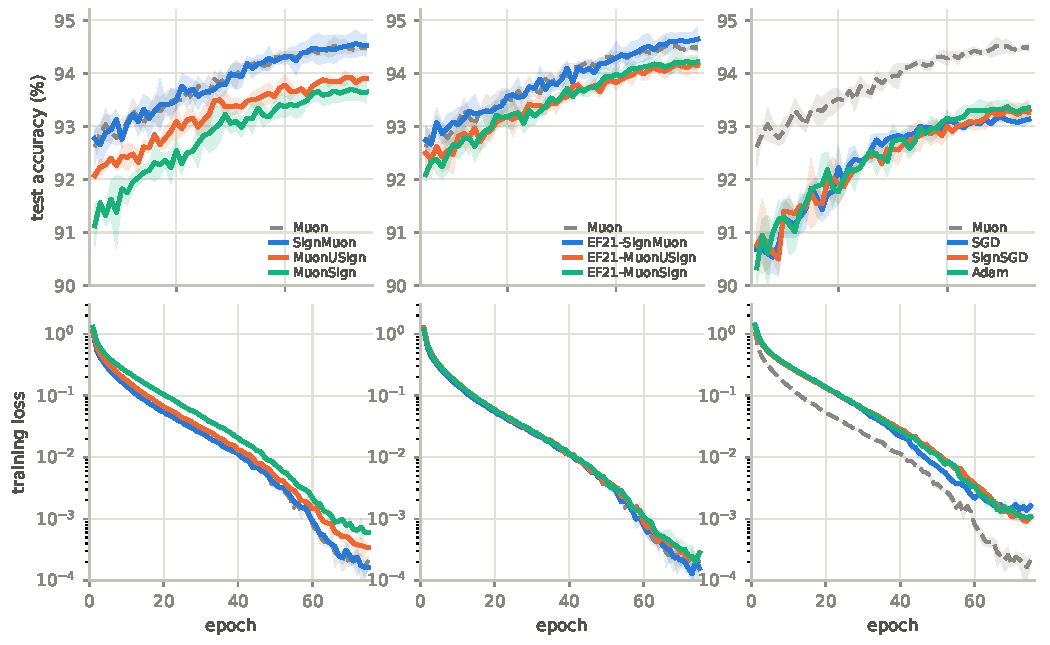
\includegraphics[width=\textwidth]{images/centralized_images/cifar_main.pdf}
    \caption{Centralized ResNet-18 on CIFAR-10: test accuracy from epoch $25$, at each method's selected $\eta_0$ (Table~\ref{tab:cifar_main}). Panels group the three sign placements (left), the EF21 variants (centre) and the uncompressed baselines (right); Muon is the gray dashed reference in all three, and bands are $\pm1$ standard deviation over three seeds.}
    \label{fig:cifar_results}
\end{figure*}

We compare all six matrix-aware 1-bit methods against Muon, SignSGD, SGD and Adam at a fixed epoch budget, on CIFAR-10 \cite{krizhevsky2009cifar}. The base model is a ResNet-18 adapted to low-resolution images: an initial $3\times3$ convolution without max-pooling, $4$ residual blocks with BatchNorm, dropout, and a linear classifier. Training runs for $T_{\max}=75$ epochs with $\eta_0$ annealed to zero by a cosine schedule.

\paragraph{Protocol.} The only tuned hyperparameter is $\eta_0$, selected per method on a held-out $5$k validation split. Every method with a norm-fixed step is tuned and reported under one per-layer rule, the unit-gain rule~\eqref{eq:unit_gain_main}, so that $\eta_0$ means the same thing across them, namely the per-step RMS gain (Appendix~\ref{app:lrscale}); SGD and Adam have no such step and keep one global rate. Centralized numbers are means over three seeds and federated numbers over five, and differences smaller than the seed spread are not claimed as results. Alongside final accuracy we report epochs to a fixed test accuracy, which separates the methods by factors rather than by tenths of a point. The grid, the endpoint rule and the schedules are in Appendix~\ref{app:repro}.

\begin{table}[!t]
\centering
\small
\renewcommand{\arraystretch}{1.15}
\begin{tabular}{|l|c|c|c|}
\hline
\textbf{Method} & $\boldsymbol{\eta_0}$ & \textbf{Test acc (\%)} & \textbf{Ep.\ to $\mathbf{90\%}$} \\
\hline
EF21-SignMuon & $0.01$ & $94.64 \pm 0.24$ & $8.7$ \\
SignMuon & $0.02$ & $94.53 \pm 0.22$ & $8.3$ \\
Muon & $0.05$ & $94.49 \pm 0.09$ & $7.7$ \\
\hline
EF21-MuonSign & $0.01$ & $94.22 \pm 0.13$ & $10.3$ \\
EF21-MuonUSign & $0.2$ & $94.15 \pm 0.16$ & $8.7$ \\
MuonUSign & $0.02$ & $93.90 \pm 0.08$ & $10.0$ \\
MuonSign & $0.005$ & $93.65 \pm 0.21$ & $15.0$ \\
\hline
Adam & $0.0005$ & $93.35 \pm 0.15$ & $18.8$ \\
SignSGD & $0.002$ & $93.27 \pm 0.16$ & $19.0$ \\
SGD & $0.02$ & $93.13 \pm 0.07$ & $21.7$ \\
\hline
\end{tabular}
\caption{Centralized ResNet-18 / CIFAR-10, $75$ epochs. Test accuracy is the mean $\pm$ standard deviation over three seeds of the last five epochs; ``Ep.\ to $90\%$'' is the mean epoch at which test accuracy first reaches $90\%$. Rules separate the statistically tied methods from the rest.}
\label{tab:cifar_main}
\end{table}

EF21-SignMuon, SignMuon and Muon span $0.15$ points against seed spreads of $0.09$--$0.24$; at three seeds they are indistinguishable, so we claim only that sign-after \emph{matches} Muon, at one bit per parameter on the uplink and $1.26$ points above SignSGD, which spends the same budget without the \textsc{lmo}. Error feedback incurs no measurable cost here: EF21-SignMuon lies within a seed spread of uncompressed SignMuon.

Within the family the ordering exceeds the noise: sign-after ($94.53$), sign-before ($93.90$) and bidirectional ($93.65$) separate by $0.9$ points, and the training loss orders them identically (Figure~\ref{fig:cifar_train_loss}), so the gap is in optimization rather than regularization. SignMuon crosses $90\%$ in $8.3$ epochs against SGD's $21.7$, SignSGD's $19.0$ and Adam's $18.8$; orthogonalization costs about $18\%$ more per epoch ($14.4$ vs.\ $12.2$\,s, one device throughout), so $2.6\times$ fewer epochs is still $2.2\times$ in wall clock.

\subsection{Federated Learning}
\begin{table}[!t]
\centering
\footnotesize
\setlength{\tabcolsep}{3pt}
\renewcommand{\arraystretch}{1.1}
\begin{tabular}{@{}lccccc@{}}
\toprule
\textbf{Optimizer} & $\boldsymbol{\eta_0}$ & \textbf{Up} & \textbf{Down} &
\begin{tabular}[b]{@{}c@{}}\textbf{Rds.\ to}\\$\mathbf{80\%}$\end{tabular} &
\begin{tabular}[b]{@{}c@{}}\textbf{Test acc}\\\textbf{(\%)}\end{tabular} \\
\midrule
Muon & $0.1$ & $32$ & $32$ & $260$ & $85.99 \pm 0.26$ \\
SignMuon & $0.05$ & $\mathbf{1.09}$ & $\mathbf{1.09}$ & $300$ & $85.81 \pm 0.25$ \\
EF21-SignMuon & $0.05$ & $\mathbf{1.09}$ & $32$ & $600$ & $85.16 \pm 0.15$ \\
MuonUSign & $0.05$ & $\mathbf{1.09}$ & $32$ & $540$ & $84.62 \pm 0.17$ \\
EF21-MuonSign & $0.05$ & $\mathbf{1.09}$ & $\mathbf{1.09}$ & $980$ & $83.99 \pm 0.28$ \\
EF21-MuonUSign & $0.05$ & $\mathbf{1.09}$ & $32$ & $1000$ & $83.75 \pm 0.21$ \\
SignSGD & $0.02$ & $\mathbf{1.09}$ & $\mathbf{1.09}$ & $1080$ & $81.83 \pm 0.43$ \\
MuonSign & $0.05$ & $\mathbf{1.09}$ & $\mathbf{1.09}$ & $1300^{\dagger}$ & $80.68 \pm 1.88$ \\
SGD & $0.1$ & $32$ & $32$ & $1367^{\dagger}$ & $79.79 \pm 1.55$ \\
Adam & $0.001$ & $32$ & $32$ & --- & $77.12 \pm 1.04$ \\
\bottomrule
\end{tabular}
\caption{CIFAR-10 federated learning on CNN2, ordered by accuracy: $N=11$ clients, homogeneous split, $2000$ rounds at batch $192$ per client, momentum $0.9$. Test accuracy is the mean of the final five evaluations over five seeds, $\pm$ one standard deviation \emph{across} seeds. \textbf{Up} and \textbf{Down} are mean bits per model parameter per round in each direction (Appendix~\ref{app:commacct}). $^{\dagger}$~mean over the seeds reaching $80\%$ within the budget ($4/5$ for MuonSign, $3/5$ for SGD); Adam reached it on none.}
\label{tab:exp_3}
\end{table}

In federated learning the bottleneck is transmitting full $32$-bit gradient matrices. We compare all six matrix-aware 1-bit methods against the Muon, SignSGD, SGD and Adam baselines on CNN2 (two convolutional blocks with BatchNorm and an MLP classifier), with CIFAR-10 partitioned homogeneously across clients. Local models are discarded at the end of each round, so BatchNorm runs at its initialization statistics throughout, in training and evaluation alike (Appendix~\ref{app:repro}). Two schemes are covered: the worker-side-LMO scheme (Algorithm~\ref{alg:fed_workerlmo}), of which federated SignMuon is the instance, and the server-side-LMO scheme (Algorithm~\ref{alg:fed_serverlmo}), which covers the error-feedback variants; Table~\ref{tab:fed_master} lists which compressor pair fixes each method.

\paragraph{Setting.} Sign-based methods separate most clearly as network scale and local computation grow, so we run at $N=11$ clients at batch $192$ each, the scale at which they separate. Clients take no local parameter steps. The count is odd by design: client messages are $\pm1$ valued under the convention of Section~\ref{sec:theory}, so an odd $N$ makes the majority vote decisive in every coordinate and removes the tie-breaking rule from the comparison entirely. Every rate is tuned per method on a validation split held out before the client partition, so that no placement is handicapped by its step size and no test image is scored during selection (Appendix~\ref{app:repro}); every number is a five-seed mean (Table~\ref{tab:exp_3}, Figure~\ref{fig:exp_3}).

SignMuon reaches the quality of Muon at $1.09$ bits per parameter in \emph{both} directions, a gap of $0.18$ points against a seed spread of $0.25$. At that fixed one-bit round trip, replacing the gradient sign with the sign of the \textsc{lmo} direction is worth $3.98$ points over SignSGD, against $1.26$ centrally. The seeds also separate the three placements, which single-seed evidence had shown as coincident: sign-after leads, sign-before trails it by $1.19$ points, and signing both sides costs a further $3.94$. Sign-after stays ahead under error feedback, though below it the other two swap.

This is the paper's uncomfortable finding: the placement that works best in practice is the one the theory condemns. Sign-after is what Theorem~\ref{th:1} makes diverge, and error feedback does not repair it for any $(L,\eta,\mu)$ (Theorem~\ref{th:ef_div}); yet the sign-after methods are the strongest compressed ones here, in the centralized table, and on nanoGPT (Section~\ref{sec:exp_nanogpt}). Conversely the two variants carrying an unconditional $\mathcal{O}(T^{-1/2})$ guarantee lie about $2$ points below SignMuon, seven to eight seed spreads. The guarantee therefore costs accuracy at this scale, and the counterexamples constrain worst-case instances rather than predicting CIFAR-10.

EF21-MuonSign is $0.24$ points \emph{ahead} of the uplink-only EF21-MuonUSign, within a seed spread, so at CNN2's scale the one-bit downlink loop incurs no measurable cost: what separates the EF21 family from SignMuon is the sign placement, not the second compression. All methods are evaluated at the exact server model $\mathbf{X}_t$, the iterate Corollary~\ref{cor:smooth} bounds, which for EF21-MuonSign is not the model the clients hold \eqref{eq:two_models}; that the two agree here means the models still track each other. On much wider matrices they separate (Remark~\ref{rem:dimension}), and the next section reports both.

\subsection{Language Modelling}\label{sec:exp_nanogpt}

\begin{figure}[!t]
\centering
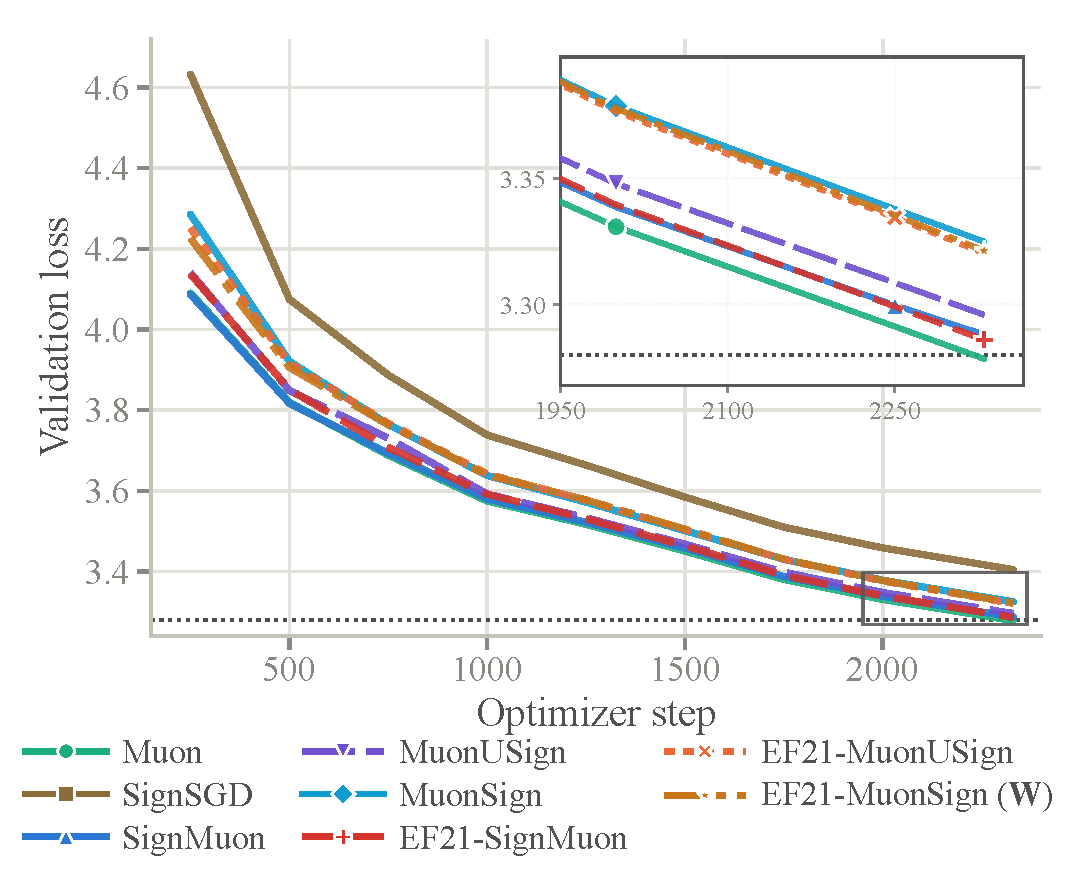
\includegraphics[width=\columnwidth]{images/nanogpt/fig_nanogpt_main.pdf}
\caption{NanoGPT speedrun, $8\times$H100: validation loss against optimizer step, single seed; dotted is the speedrun target $3.28$. EF21-MuonSign is drawn at its broadcast model $\mathbf{W}$. The inset magnifies the boxed tail, where SignSGD is above the range shown; exact values are in Table~\ref{tab:nanogpt}.}
\label{fig:nanogpt}
\end{figure}

\begin{table}[!t]
\centering\small
\setlength{\tabcolsep}{4pt}
\begin{tabular}{@{}llccc@{}}
\toprule
\textbf{Method} & \textbf{Step} & $\boldsymbol{\eta_0}$ & \textbf{Val.\ loss} & \textbf{Steps to $3.35$} \\
\midrule
Muon (record \#40)   & \textsc{lmo}  & 0.06 & \textbf{3.2785} & $1.00\times$ \\
EF21-SignMuon        & \textsc{lmo}  & 0.06 & 3.2860 & $1.02\times$ \\
SignMuon             & \textsc{sign} & 0.03 & 3.2881 & $1.02\times$ \\
MuonUSign            & \textsc{lmo}  & 0.06 & 3.2959 & $1.05\times$ \\
EF21-MuonUSign       & \textsc{lmo}  & 0.06 & 3.3203 & $1.13\times$ \\
EF21-MuonSign ($\mathbf{W}$) & \textsc{lmo} & 0.06 & 3.3213 & $1.14\times$ \\
MuonSign             & \textsc{sign} & 0.03 & 3.3249 & $1.14\times$ \\
SignSGD              & \textsc{sign} & 0.03 & 3.4049 & -- \\
\midrule
EF21-MuonSign ($\mathbf{X}$) & \textsc{lmo} & 0.06 & 5.5198 & -- \\
\bottomrule
\end{tabular}
\caption{NanoGPT after $2330$ steps ($611$M tokens), single seed. Record \#40 reports $3.2780\pm0.0009$ over five seeds, so differences below ${\sim}0.003$ are noise. ``Steps to $3.35$'' is the step count to reach that loss, relative to Muon. The last row is EF21-MuonSign's server model $\mathbf{X}$, the same run as the broadcast model $\mathbf{W}$ above.}
\label{tab:nanogpt}
\end{table}

We test the methods where the matrices are large enough for the layer-rank dependence of Corollary~\ref{cor:smooth} to take effect: the modded-nanoGPT speedrun (record \#40), a $12$-layer transformer of model dimension $768$ with $768\times3072$ hidden matrices, trained on $611$M FineWeb tokens on $8\times$H100. Each method replaces the record's Muon on the hidden matrices and gates; embeddings, scalars and the head keep the record's Adam. Our Muon arm \emph{is} record~\#40's own optimizer and reproduces its published result to $0.6$~sd, which validates the port before anything else is read. Rates are not tuned per method but fixed a priori by the unit-gain rule at one $\eta_0$ per \emph{family} ($0.06$ for the \textsc{lmo}-terminated methods, the record's own value, and $0.03$ for the \textsc{sign}-terminated ones), so every contrast is matched-hyperparameter, at the cost of not reporting each method's best achievable loss. Runs are single-seed, and Table~\ref{tab:nanogpt} states the seed noise of the reference so that the resolvable differences are explicit (Appendices~\ref{app:nanogpt} and~\ref{app:lrscale}).

Three things follow (Table~\ref{tab:nanogpt}, Figure~\ref{fig:nanogpt}). First, the matrix-aware 1-bit methods transfer to language modelling: all of them beat SignSGD by $0.08$--$0.12$ nats, and the best of them lie within $0.01$ of full-precision Muon, at equal wall-clock. Second, error feedback is inexpensive but not without cost. Its clean cost is the matched pair MuonUSign\,$\to$\,EF21-MuonUSign, $+0.024$ nats or ${\sim}8\%$ more steps, the cost of steering the LMO with an estimator that lags its target. EF21-SignMuon, whose target $\operatorname{polar}(\tilde{\mathbf{M}}_t)$ is orthogonal and hence isotropic, incurs almost no cost and is the strongest compressed method here, notwithstanding Theorem~\ref{th:ef_div}.

Third, the bidirectional method's two models \eqref{eq:two_models} come apart here. Its broadcast model $\mathbf{W}$ --- the one every gradient is evaluated at --- is indistinguishable from EF21-MuonUSign ($3.3213$ vs $3.3203$), so the compressed \emph{downlink} incurs no measurable cost where training happens. The server model $\mathbf{X}$, which is what Corollary~\ref{cor:smooth} bounds, settles ${\approx}2.2$ nats above it: a persistent offset, not a divergence, and one that Appendix~\ref{app:nanogpt} localizes to the single zero-initialized $\mathtt{c\_proj}$ layer. This is the mechanism of Remark~\ref{rem:dimension} rather than a tuning failure, and lowering $\eta_0$ does not repair it, since the admissible step would have to shrink by a further $\sqrt{r}$ in the layer rank (Remark~\ref{rem:normmismatch}). A spectrally contractive downlink compressor would repair it.

\section{Conclusion}\label{sec:conclusion}


SignMuon applies 1-bit sign compression to the Muon LMO direction: it matches Muon's accuracy and outperforms SignSGD, but we prove that a directly sign-compressed LMO has no global convergence guarantee and can diverge. EF21-MuonUSign compresses the internal residual instead, which restores a transferred $\mathcal{O}(T^{-1/2})$ guarantee and descent on our counterexamples at a 1-bit uplink, and remains about two accuracy points below uncompressed SignMuon; EF21-MuonSign brings the downlink to one bit at no measured cost.

An open tension remains. On every task we measure (centralized, federated and language modelling), the strongest compressed method places the sign after the LMO, exactly the placement Theorems~\ref{th:1} and~\ref{th:ef_div} show to be unrepairable in the worst case. The practitioner chooses between a bound that holds on every instance and roughly two accuracy points on the instances they have; narrowing that gap, by finding what property of realistic problems the counterexamples violate, is the natural continuation of this work.
\paragraph{Future work.} Our $(L^0,L^1)$ guarantee (Corollary~\ref{cor:l0l1}) covers the uplink-compressed EF21-MuonUSign only, since the generalized-smooth theory of \citet{gruntkowska2025error} is available only without downlink compression; extending it to EF21-MuonSign is open. So is the downlink itself: the rank penalty EF21-MuonSign incurs comes from compressing the model in the wrong norm, removable only by changing the compressor (Remark~\ref{rem:normmismatch}), and whether \emph{any} one-bit compressor can be layer-norm contractive we do not know. Since \citet{gruntkowska2025error} fix the server compressor to the identity throughout their experiments, this regime appears not to have been probed empirically before. The most useful question our results leave open, though, is whether sign-after can be repaired. It is the placement practitioners would pick and the one we cannot certify, so it is at present a working heuristic; what our counterexamples rule out is a guarantee holding on \emph{every} instance, not one holding under an assumption realistic problems satisfy, and identifying such an assumption would close the gap this paper documents. Finally, the reduction of Appendix~\ref{app:hyp} applies verbatim to arbitrary layer geometries (Remark~\ref{rem:gluon}), and how these methods scale to LLM-sized matrices remains to be measured.

%%%%%%%%%%%%%%%%%%%%%%%%%%%%%%%%%%%%%%%%%%%%%%%%%%%%%%%%%%%%
% References (placed after the Appendix; see note above).
% \bibliographystyle{unsrtnat}  % aaai2027.sty sets the style to aaai2027.bst automatically

% \bibliographystyle{unsrtnat}  % aaai2027.sty sets the style automatically
